\documentclass{article}

\usepackage[utf8]{inputenc}
\usepackage{tikz}
\usepackage{verbatim}
\usepackage{array}
\newcolumntype{P}[1]{>{\centering\arraybackslash}p{#1}}
\usepackage[utf8]{inputenc}
\usepackage{natbib}
\usepackage{graphicx}
\usetikzlibrary{arrows,calc}
\usepackage{relsize}

\renewcommand{\arraystretch}{1.5}

\setlength{\parindent}{0em}
\setlength{\parskip}{1em}

\title{ACALA Token Economy Working Paper}
\author{Antonia Chen}
\date{4 Nov 2019}

\begin{document}

\maketitle


\section{Key Functions of ACA Token}
ACA is the native token of ACALA Network. ACAs serve three key functions in ACALA Network:

\begin{itemize}
    \item \textbf{Utility Token} \\
    To close any CDP that has been created to generate aUSDs in the ACALA Network, some ACA tokens are required to be paid as the Stability Fee (Equivalent amount of aUSDs is also accepted by the official portal and will be exchanged to ACA automatically).
    
    When ACA is received, it is burned and removed from the supply permanently. As market demand for aUSDs and CDPs increase, demand for ACA increase as users need them to pay the Stability Fee. 
    
    \item \textbf{Governance of the Network} \\
    As a governance token, ACA tokens provide their holders voting right for the risk management and business logic of the ACALA Network, including adjustment of risk parameters, such as Stability fee, Debt Ceiling, Liquidation Ratio and Liquidation Penalty. 

    \item \textbf{Contingency Solution} \\
     In situations such as a sudden price crash of collateral token resulting in insolvency of under-collateralized CDPs, ACA will be automatically diluted and sold on market for system recapitalization.
    
\end{itemize}

\section{Minting and Distribution of ACA Tokens}
The total supply of $A$ unit of ACA Tokens will be minted at the launch of the mainnet and stored in the ACA Reserve Pool to be distributed to:

\begin{itemize}
    \item \textbf{ACALA Foundation} \\
    45\% will be reserved by the ACALA Foundation at launch, which will be distributed to the ACALA Foundation, Ecosystem Development, Future Key Investment Partners through time.
    
    \item \textbf{Seed Investment Partners} \\
    10\% will be distributed to the initial investment partners in the Seed Investment Round.

    \item \textbf{As Reward to IPO Participants} \\
    30\% will be distributed to IPO participants with detailed proposal in Section 7.
    
    \item \textbf{Be Sold to the public} \\
    15\% are available to be distributed to the public with detailed proposal in Section 8.
     
\end{itemize}

Unless required as a contingency solution, no more ACA token will be minted afterward the launch of mainnet.


\section{Burning of ACA Tokens}

\begin{itemize}
    \item \textbf{Stability Fee} \\
    To close a CDP with outstanding debt of $n$ aUSDs, the CDP owner is required to pay $s \cdot n$ aUSDs worth of ACA tokens as Stability Fee, where $s$ is the Stability Fee rate, e.g. 5\%. Once received, the ACA tokens will be automatically burnt by the system and permanently removed from the ACA supply.  
    
    \item \textbf{Liquidation Penalty} \\
    All open CDPs are constantly monitored by the system, and for each type of collateral, ACA holders vote a liquidation ratio - a certain limit that the amount of overcollaterization a CDP requires to meet to avoid liquidation.  
    
    Once the value of the CDP collateral has fallen below the liquidation ratio, then the CDP becomes risky and is automatically liquidated by the system in a Collateral Auction mechanism. 

    The Collateral Auction is designed to operate in two phrases to be fair to CDP owners that only the part of collateral that is enough to cover both the outstanding debt in the CDP and a liquidation penalty of $p \cdot n$ (e.g. $p=10\%$) aUSDs will be sold, with the remaining returned to the CDP original owners. 
    
    The liquidation penalty will be automatically used to purchase ACA tokens in external exchange by the system, which will be burnt and permanently removed from the ACA supply.  
     
\end{itemize}

\section{Parachain Auction}
We plan to launch our mainnet on a Parachain slot, to be leased from Polkadot, using DOTs to be crowdfunded. A specially designed Candle Auction is utilized to sell the leasing right of Parachain slots. It is a mechanism designed for fairness, e.g. to prevent early sniping and provide bidders with higher valuation higher chances of winning. Since it will be a challenge to estimate private valuation distribution of bidders with private bidding strategies, and we plan to conduct a Crowdfund IPO (Initial Parachain Offering), that we will:

    \begin{enumerate}
    \item Start our DOT Crowdfund at time $t-30$  
    \item Bid $W^1_0$ - total fund collected for a 24-month lease of a Parachain slot, at time $0$, the open time of the first Parachain slot auction
    \item Bid $W^1_t$ whenever total fund increase at time $t<T$, before the close time $T$ of the first Parachain slot auction
    \item After the retroactive close time $t^*$ of the first Parachain slot auction is announced, if our last bid before $t^*$ is successfully accepted, $W^1_{t^*}$  unit of DOTs will be locked to lease the Parachain slot and the rest of $W^1_{T} - W^1_{t^*}$ DOTs that are deposited into the crowdfund after $t^*$ will be returned to their owners,
    \item Distribute ACA tokens as rewards to DOT owners who participate our first IPO successfully, to compensate their opportunity costs of having their DOTs locked for 24 months, with detailed proposal in Section 7. 
    \end{enumerate}


\section{Parathreads}
In case our first Parachain slot auction was not successful, we will continue to launch our mainnet on Parathreads instead. DOTs raised in IPO will be returned to their owners, and ACA tokens will still be minted at launch, but only distributed to ACALA Founders and Seed Investment Partner according to the original plan, with the rest reserved for future investment opportunities including IPO in the second Parachain auction. 

Compared to Parachain, there are gas costs using Parathreads, depending on frequency of validation. The more frequent a validation is processed, the safer the network is, at a price of higher gas costs. ACA holders will vote to determine the frequency. A small amount of ACA tokens will be released from the reserve and sold to public for DOTs daily to cover the entire gas costs of the network daily validation. For say, if the total gas costs are estimated to be 5 ACA tokens worth of DOTs for the day, 5 ACA tokens will be released and sold by the system. Another IPO will be raised to lease a Parachain slot before the second Parachain auction. 

\section{Three Rounds of Parachain Lot Lease}
We plan to lease the Parachain slot for three rounds of six years (24 months in each round), in hope to switch to our independent blockchain bridging to Polkadot after 6 years. 

Assuming that DOTs are estimated to generate a net effective annual return of $r$ (profit margin of being a validator with all cost deducted, e.g. 10\%), and we have $30\% \cdot A$ unit of ACA tokens to be distributed to IPO participants in the three rounds as reward for locking their DOTs for our lease of Parachain slot. 

\subsection{Ideal Situation}

In ideal situation, when relative cost of leasing a Parachain do not fluctuate significantly among Parachain leasing periods. Suppose we won our first Parachain auction at cost of $W^1_{t^*}$ that the estimated costs of leasing the same slot at the second round and third round are  $W^1_{t^*} (1+r)^2$ and  $W^1_{t^*}(1+r)^4$  respectively. all ACA tokens in the IPO Reward Reserve are distributed to IPO participants in the three IPOs accordingly that there will be zero ACA token left by the end of the third round of lease (six years after launch). The ACALA network is expected to be ready to upgrade to an independent blockchain bridging to Polkadot by then, and all ACA holders will be invited to vote whether to upgrade to independent blockchain or lease another round of Parachain slot by minting more ACA tokens as rewards for the fourth-round IPO participants. 

\begin{center}
\begin{tabular}{ |P{1.2cm}||P{4.3cm}|P{2.5cm}|P{2.2cm}|}
 \hline
 \multicolumn{4}{|c|}{Three Rounds of Parachain Lot Lease (Ideal Situation)} \\
 \hline
   Round & Winning Bid & Proportion in Reward Reserve & ACA Rewards when $r=10\%$\\
 \hline
1 & $W^1=W^1_{t^*}$   & $\frac{1}{1+(1+r)^2+(1+r)^4}$ & $8.17\% \cdot A$ \\[2ex]
2 & $W^2 = W^1(1+r)^2$   & $\frac{(1+r)^2}{1+(1+r)^2+(1+r)^4}$ & $9.88\% \cdot A$  \\[2ex]
3 & $W^3 = W^1(1+r)^4$   & $\frac{(1+r)^4}{1+(1+r)^2+(1+r)^4}$ & $11.95\% \cdot A$  \\[2ex]
 \hline
Total & $W=W^1+W^2+W^3=$ $W^1[1+(1+r)^2+(1+r)^4]$    &  {100\%}   & {$30\% \cdot A$} \\
 \hline
\end{tabular}
\end{center}

However, extreme cases are not uncommon in the world of blockchains, that all possible scenarios (categorised into four special cases as below) are analysed. 


\subsection{Special Case I}
In situations when rapid growth of the Polkadot network cause exploding demand of the Parachain slots, that $W^2$ winning bid in the second round of Parachain auction is much higher than $W^1$. When
$$W^2 > W^1[(1+r)^2 + (1+r)^2]$$
the system will distribute all remaining ACA tokens in the IPO Reward Reserve 
$$ \frac{(1+r)^2+(1+r)^4}{1+(1+r)^2+(1+r)^4} \cdot 30\% A  $$
to IPO participants in the second round. For instance, when $W^2=5W^1$, all remaining ACA tokens in IPO Reward Reserve are distributed in the second round. 

Therefore, we have zero ACA tokens left in reward reserve for IPO participants in the third round. Given the trend of growth, it is very likely that by the end of the second round of lease (four years after launch), the ACALA network will be ready to upgrade to an independent blockchain bridging to Polkadot, rather than leasing a Parachain slot. All ACA holders will be invited to vote whether to upgrade to independent blockchain or lease another round of Parachain slot by minting more ACA tokens as rewards for the third-round IPO participants. 

\begin{center}
\begin{tabular}{ |P{1.2cm}||P{4.3cm}|P{2.5cm}|P{2.2cm}|}
 \hline
 \multicolumn{4}{|c|}{Three Rounds of Parachain Lot Lease (Special Case I)} \\
 \hline
   Round & Winning Bid & Proportion in Reward Reserve & ACA Rewards when $r=10\%$\\
 \hline
1 & $W^1=W^1_{t^*}$   & $\frac{1}{1+(1+r)^2+(1+r)^4}$ & $8.17\% \cdot A$ \\[3ex]
2 & $W^2 > W^1[(1+r)^2 + (1+r)^2]$   & $\frac{(1+r)^2+(1+r)^4}{1+(1+r)^2+(1+r)^4}$ & $ 21.87\% \cdot A $  \\[3ex]
3 & Strategy to be Voted   & TBV & TBV  \\[1ex]
 \hline
Total & $W$    & TBV   & TBV \\
 \hline
\end{tabular}
\end{center}

\vspace{5mm}


\subsection{Special Case II}
In situations when growth of the Polkadot network is faster than expectation and cause increasing demand of the Parachain slots, that $W^2$ winning bid in the second round of Parachain auction is higher than expectation, but not as extreme as in Special Case I. When
$$W^1(1+r)^2 < W^2 < W^1[(1+r)^2 + (1+r)^2]$$
the system will distribute a proportion of remaining ACA tokens in the Reward Reserve with respect to ratio of $W^2$ and $W^1$ 
$$\frac{W^2/W^1}{1+(1+r)^2+(1+r)^4} \cdot 30\% A  $$
to IPO participants in the second round. For instance, when $W^2=2W^1$, reward ACA tokens distributed in the second round are doubled compared to the first round. 

Therefore, we have a lot less ACA tokens left in reward reserve for IPO participants in the third round, compared to the ideal situation. Given the trend of growth, it is likely that by the end of the second round of lease (four years after launch), the ACALA network will be ready to upgrade to an independent blockchain bridging to Polkadot, rather than leasing a Parachain slot. All ACA holders will be invited to vote whether to upgrade to independent blockchain or lease another round of Parachain slot by minting more ACA tokens as rewards for the third-round IPO participants. 

\begin{center}
\begin{tabular}{ |P{1.2cm}||P{4.3cm}|P{2.5cm}|P{2.2cm}|}
 \hline
 \multicolumn{4}{|c|}{Three Rounds of Parachain Lot Lease (Special Case II)} \\
 \hline
   Round & Winning Bid & Proportion in Reward Reserve & ACA Rewards when $r=10\%$\\
 \hline
1 & $W^1=W^1_{t^*}$   & $\frac{1}{1+(1+r)^2+(1+r)^4}$ & $8.17\% \cdot A$ \\[3ex]
2 & $W^2 > W^1(1+r)^2$   & $\frac{W^2/W^1}{1+(1+r)^2+(1+r)^4}$ & $ 8.17\% \cdot A \frac{W^2}{W^1}$  \\[3ex]
3 & Strategy to be Voted   & TBV & TBV  \\[1ex]
 \hline
Total & $W$    & TBV   & TBV \\
 \hline
\end{tabular}
\end{center}

\vspace{5mm}

\subsection{Special Case III}
In situations when demand of the Parachain slots somehow shrink extremely due to unexpected problems, that winning bids in the second and other future round of Parachain auction becomes super small or zero that it is free to lease a Parachain slot. When
$$W^i =0 \quad \forall i>1$$
the system will NOT distribute any remaining ACA tokens in the IPO Reward Reserve. All ACA holders may vote to decide whether to use these tokens for other purposes such as raising investment or burn them to remove permanently from the ACA supply.

\begin{center}
\begin{tabular}{ |P{1.2cm}||P{4.3cm}|P{2.5cm}|P{2.2cm}|}
 \hline
 \multicolumn{4}{|c|}{Three Rounds of Parachain Lot Lease (Special Case III)} \\
 \hline
   Round & Winning Bid & Proportion in Reward Reserve & ACA Rewards when $r=10\%$\\
 \hline
1 & $W^1=W^1_{t^*}$   & $\frac{1}{1+(1+r)^2+(1+r)^4}$ & $8.17\% \cdot A$ \\[2ex]
2 & $W^2 = 0$   & 0\% & 0  \\[1ex]
3 & $W^3 = 0$   & 0\% & 0  \\[1ex]
 \hline
Total & $W=W^1+0+0=W^1$    &  {100\%}   & {$30\% \cdot A$} \\
 \hline
\end{tabular}
\end{center}

\vspace{5mm}

\subsection{Special Case IV}
In situations when demand of the Parachain slots somehow do not grow as fast as expected in ideal situation or shrink, that winning bids in the second and other future round of Parachain auction is smaller than expectation in ideal situation. When
$$0<W^2 < W^1(1+r)^2$$
the system will distribute a proportion of remaining ACA tokens in the Reward Reserve with respect to ratio of $W^2$ and $W^1$ 
$$\frac{W^2/W^1}{1+(1+r)^2+(1+r)^4} \cdot 30\% A  $$
to IPO participants in the second round. For instance, when $W^2=0.5 W^1$, reward ACA tokens distributed in the second round will only be half as many compared to the first round. 

If the weak trend in demand of Parachain slots continue that we will more ACA tokens left in the IPO Reward Reserve by the end of the second round of lease, than expected in ideal situation. When
$$0<W^3 < W^1[(1+r)^2+(1+r)^4] - W^2$$
the system will distribute a proportion of remaining ACA tokens in the Reward Reserve with respect to ratio of $W^3$ and $W^1$ 
$$\frac{W^3/W^1}{1+(1+r)^2+(1+r)^4} \cdot 30\% A  $$
to IPO participants in the second round. For instance, when $W^3=0.75 W^1$, reward ACA tokens distributed in the second round will only be three quarters as many compared to the first round. 

Therefore, we still have some ACA tokens left in the IPO reward reserve after the end of the third round lease. If there are enough to reward IPO participants in the fourth round, the system will distribute them the same way as in previous two rounds. If there are not enough ACA tokens left, all ACA holders will be invited to vote whether to mint more ACA tokens as rewards to run a fourth IPO. 

\begin{center}
\begin{tabular}{ |P{1.2cm}||P{4.3cm}|P{2.5cm}|P{2.2cm}|}
 \hline
 \multicolumn{4}{|c|}{Three Rounds of Parachain Lot Lease (Special Case IV)} \\
 \hline
   Round & Winning Bid & Proportion in Reward Reserve & ACA Rewards when $r=10\%$\\
 \hline
1 & $W^1=W^1_{t^*}$   & $\frac{1}{1+(1+r)^2+(1+r)^4}$ & $8.17\% \cdot A$ \\[2ex]
2 & $W^2 < W^1(1+r)^2$   & $\frac{W^2/W^1}{1+(1+r)^2+(1+r)^4}$ & $ 8.17\% \cdot A \frac{W^2}{W^1}$  \\[3ex]
3 & $W^3 < W^1[(1+r)^2+(1+r)^4] - W^2$ &  $\frac{W^3/W^1}{1+(1+r)^2+(1+r)^4}$ & $ 8.17\% \cdot A \frac{W^3}{W^1}$ \\[3ex]
 \hline
Total & TBV    & TBV   & TBV \\
 \hline
\end{tabular}
\end{center}

\section{Distribution of ACA Reward Tokens for IPOs}
The total amount of ACA Reward tokens to be distributed in each of the three round of Parachain slot lease have been discussed in the previous section, we now look at how these tokens will be distributed to the IPO participants in each round. It is obvious that the tokens would be better distributed in a frequent manner and small batches rather than in lump sums at beginning of each round, which lead to sudden large shifts in ACA supply causing unfavourable large price fluctuations as shown below. 

    \begin{center}
    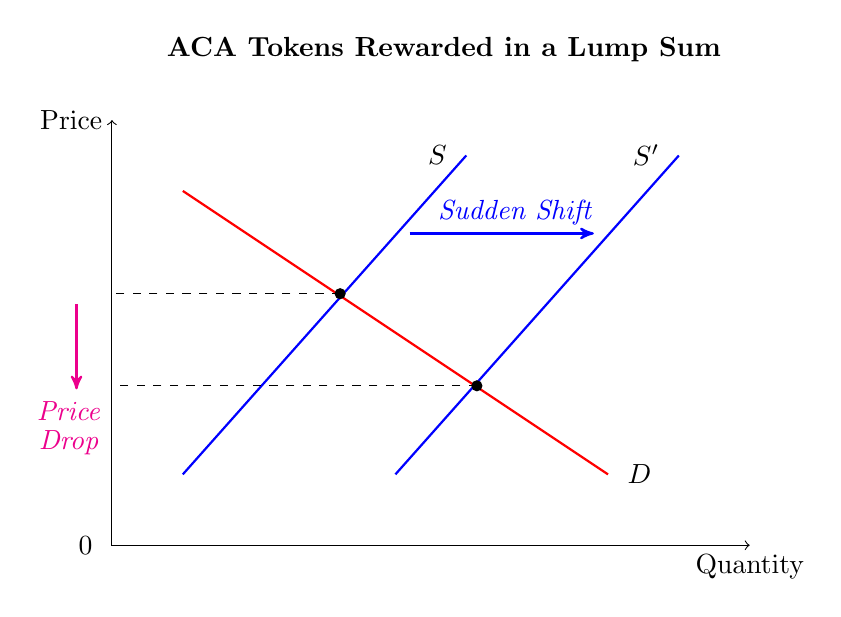
\begin{tikzpicture}[scale=0.9]

    \draw[<->] (9,0) node[below]{Quantity} -- (0,0) -- (0,6) node[left]{Price};
    \draw [thick, blue] (1,1) -- (5,5.5);
    \draw [thick, blue] (4,1) -- (8,5.5);
    \draw [thick, red] (1,5) -- (7,1);

    \filldraw[black](3.22,3.55) circle (2pt) {};
    \filldraw[black](5.15,2.25) circle (2pt) {};
   
    \draw [dashed] (3.22,3.55) -- (0,3.55);
    \draw [dashed] (5.15,2.25) -- (0,2.25);   

    \node[dotted,label=left:$0$] at (0,0) (int0) {};
    \node[dotted,label=left:$S$] at (5,5.5) (int1) {};
    \node[dotted,label=left:$S'$] at (8,5.5) (int2) {};
    \node[dotted,label=right:$D$] at (7,1) (int3) {};
    
    \node[dotted, magenta] at (-0.6,1.9) (int4) {\textit{Price}};
    \node[dotted, magenta] at (-0.6,1.45) (int5) {\textit{Drop}};
    \node[dotted, blue] at (5.7,4.7) (int6) {\textit{Sudden Shift}};

    \node[dotted,label=right:{\textbf{ACA Tokens Rewarded in a Lump Sum}}] at (0.5,7) (int7) {};
  
    \draw[->, thick, magenta, >=stealth'](-0.5,3.4) -- (-0.5,2.2);
    \draw[->, thick, blue, >=stealth'](4.2,4.4) -- (6.8,4.4);
    
    \end{tikzpicture}
    \end{center}

\vspace{1cm}

We propose that all ACA Reward tokens planned to be distributed in each round are to be distributed to each successful IPO participant at every second, according to the proportion of their shares of locked DOTs in the total number of locked DOTs. For instance, since $W^1$ DOTs are locked for lease of Parachain slot in the first round, that in every second of the first 24 months (duration of round one lease), each IPO participant receives
$$\frac{30\% A W^1}{3600 \times 24 \times 365 \times 2 \times [1+(1+r)^2+(1+r)^4]}$$
for every locked DOT he or she owns. \\

Since ACA Tokens are distributed to cover the opportunity cost of the net yield of these locked DOTs, the initial valuation of one ACA token for a IPO participant in round one is equal to
$$\frac{W^1 (1+r)^2 [1+(1+r)^2+(1+r)^4 ]}{30\% A} $$

In long run, supply of ACA tokens decrease as they are burnt by the system through receiving Stability Fees and Liquidation Penalty, which increase valuation and market price of ACA tokens. While in short run, there would exist frequent small price fluctuations following the market conditions, e.g. collateral price changes, raising demand of aUSDs and etc. 


    \begin{center}
    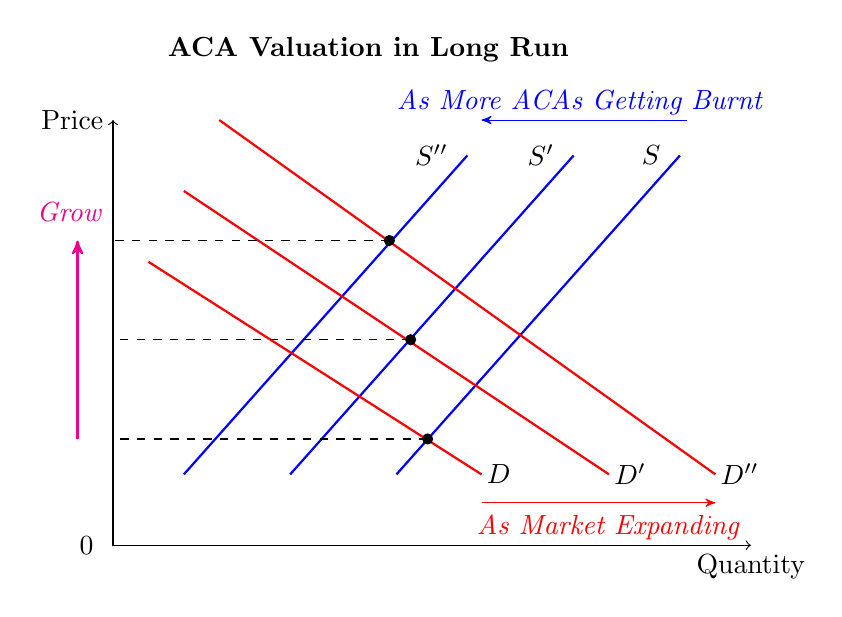
\begin{tikzpicture}[scale=0.9]

    \draw[<->] (9,0) node[below]{Quantity} -- (0,0) -- (0,6) node[left]{Price};
    \draw [thick, blue] (1,1) -- (5,5.5);
    \draw [thick, blue] (2.5,1) -- (6.5,5.5);
    \draw [thick, blue] (4,1) -- (8,5.5);
    \draw [thick, red] (1,5) -- (7,1);
    \draw [thick, red] (0.5,4) -- (5.2,1);
    \draw [thick, red] (1.5,6) -- (8.5,1);

    \filldraw[black](3.9,4.3) circle (2pt) {};
    \filldraw[black](4.2,2.9) circle (2pt) {};
    \filldraw[black](4.44,1.5) circle (2pt) {};
   
    \draw [dashed] (3.9,4.3) -- (0,4.3);
    \draw [dashed] (4.2,2.9) -- (0,2.9);   
    \draw [dashed] (4.44,1.5) -- (0,1.5);   

    \node[dotted,label=left:$0$] at (0,0) (int0) {};
    \node[dotted,label=left:$S''$] at (5,5.5) (int1) {};
    \node[dotted,label=left:$S'$] at (6.5,5.5) (int1) {};
    \node[dotted,label=left:$S$] at (8,5.5) (int2) {};
    
    \node[dotted,label=right:$D$] at (5,1) (int3) {};
    \node[dotted,label=right:$D'$] at (6.8,1) (int3) {};
    \node[dotted,label=right:$D''$] at (8.3,1) (int3) {};
    
    \node[dotted, magenta] at (-0.6,4.7) (int5) {\textit{Grow}};
    \node[dotted, blue] at (6.6,6.25) (int6) {\textit{As More ACAs Getting Burnt}};
    \node[dotted, red] at (7,0.25) (int6) {\textit{As Market Expanding}};

    \node[dotted,label=right:{\textbf{ACA Valuation in Long Run}}] at (0.5,7) (int7) {};
  
    \draw[<-, thick, magenta, >=stealth'](-0.5,4.3) -- (-0.5,1.5);
    \draw[<-,  blue, >=stealth'](5.2,6) -- (8.1,6);
    \draw[->,  red, >=stealth'](5.2,0.6) -- (8.5,0.6);
    
    \end{tikzpicture}
    \end{center}


\vspace{1cm}

    \begin{center}
    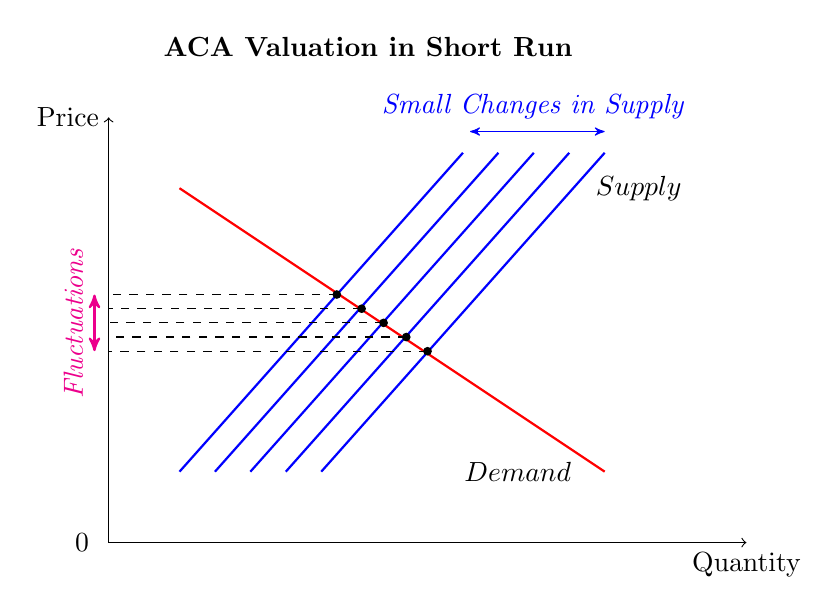
\begin{tikzpicture}[scale=0.9]

    \draw[<->] (9,0) node[below]{Quantity} -- (0,0) -- (0,6) node[left]{Price};
    \draw [thick, blue] (1,1) -- (5,5.5);
    \draw [thick, blue] (2,1) -- (6,5.5);
    \draw [thick, blue] (3,1) -- (7,5.5);
    \draw [thick, blue] (2.5,1) -- (6.5,5.5);
    \draw [thick, blue] (1.5,1) -- (5.5,5.5);
    \draw [thick, red] (1,5) -- (7,1);

    \filldraw[black](3.22,3.5) circle (1.5pt) {};
    \filldraw[black](3.57,3.3) circle (1.5pt) {};
    \filldraw[black](3.88,3.1) circle (1.5pt) {};
    \filldraw[black](4.2,2.9) circle (1.5pt) {};
    \filldraw[black](4.5,2.7) circle (1.5pt) {};
   
    \draw [dashed] (3.22,3.5) -- (0,3.5);
    \draw [dashed] (3.57,3.3) -- (0,3.3);   
    \draw [dashed] (3.88,3.1) -- (0,3.1);   
    \draw [dashed] (4.2,2.9) -- (0,2.9);
    \draw [dashed] (4.5,2.7) -- (0,2.7);

    \node[dotted,label=left:$0$] at (0,0) (int0) {};
    \node[dotted,label=right:$Supply$] at (6.6,5) (int1) {};
    
    \node[dotted,label=left:$Demand$] at (6.8,1) (int3) {};

    
    \node[dotted, magenta, rotate=90] at (-0.5,3.1) (int5) {\textit{Fluctuations}};
    \node[dotted, blue] at (6,6.15) (int6) {\textit{Small Changes in Supply}};

    \node[dotted,label=right:{\textbf{ACA Valuation in Short Run}}] at (0.5,7) (int7) {};
  
    \draw[<->, thick, magenta, >=stealth'](-0.2,2.7) -- (-0.2,3.5);
    \draw[<->, blue, >=stealth'](5.1,5.8) -- (7,5.8);
    
    \end{tikzpicture}
    \end{center}


\vspace{1cm}

\section{Distribution of ACA Tokens for Public Sale}
After a Parachain slot is secured by winning the first Parachain auction, $15\% \cdot A$ ACA tokens will be available at public sales events before the launch of mainnet, at a price set to be around the initial valuation of one ACA token for a round-one IPO participant. 

ACA tokens sold through public sales events will be distributed to the participants immediately and are ready to be traded at the launch of the mainnet. 

\section{Distribution of ACA Tokens to Other Parties}
ACA Tokens distributed to other parties such as Seed Investment Partners, are not allowed to be traded for a fixed length of time (from 12 to 24 months after launch of mainnet) for market stability. 

\end{document}